\documentclass[preprint]{elsarticle}
\usepackage[latin1]{inputenc}
\usepackage[english]{babel}
%\usepackage[T1]{fontenc}
%\usepackage{textcomp}
\usepackage{graphicx}
\usepackage{color}
%\usepackage{setspace}
\usepackage{url}

\begin{document}

\begin{frontmatter}

%%%%%%%%%%%%%%%%%%%%%%%%%%%%%%%   TITLE   %%%%%%%%%%%%%%%%%%%%%%%%%%%%%%%

\title{Nowcasting traffic}


%%%%%%%%%%%%%%%%%%%%%%%%%%%%%%%   AUTHORS   %%%%%%%%%%%%%%%%%%%%%%%%%%%%%%%

\author{A.J. Fern�ndez-Ares$^1$, A.M. Mora$^1$, M.G. Arenas$^1$, P. Garc�a-Sanchez$^1$, G. Romero$^1$, V. Rivas$^2$, P.A. Castillo$^1$, J.J. Merelo$^1$}
\ead{\{antares, amorag, mgarenas, pablogarcia, gustavo, pacv, jmerelo\}@ugr.es, vrivas@ujaes.es}
\address{$^1$ Departamento de Arquitectura y Tecnolog�a de Computadores.\\ ETSIIT - CITIC. University of Granada, Spain\\
$^2$ Departamento de Inform�tica. EPS. Universidad de Ja�n, Spain}


\begin{abstract}
Traffic flow measurement methods suffer must keep a balance between being comprehensive, expensive and cumbersome, such as traffic spirals, or being cheap, mobile but missing some counts.
In the framework of a smart city project, our group has been
developing MOBYWIT, a device that detects unique Bluetooth and Wifi
MACs and thus is able to measure their traffic, but also to identify
uniquely bearers so that we can find out the actual path a particular
vehicle has followed. However, not all vehicles have bluetooth devices
and the relation between them and the actual number of vehicles varies
along the day, the time of the day and characteristics of the road. 
In this work our objective is to "nowcast", that is, to predict, using
all available information, the real number of vehicles given that we
have the number of vehicles bearing a wireless device. We will use
classic and neural network techniques on data gathered in
installations where we have both kind of devices, MOBYWIT and spirals,
to try and find out some rules and give a more accurate estimate of
the real number of cars in a particular road. 
\end{abstract}

%
%%%%%%%%%%%%%%%%%%%%%%%%%%%%%%%%%   KEYWORDS   %%%%%%%%%%%%%%%%%%%%%%%%%%%%%%%%%
%
\begin{keyword}
Smart traffic \sep Transit indicators \sep Traffic forecast \sep Mobility analysis \sep Smart City \sep Internet of Things
\end{keyword}

\end{frontmatter}


%-------------------------------------------------------------------------------
%%%%%%%%%%%%%%%%%%%%%%%%%%%%%%%   INTRODUCTION   %%%%%%%%%%%%%%%%%%%%%%%%%%%%%%%
%-------------------------------------------------------------------------------

\section{Introduction}
\label{sec:intro}


The rest of the work is structured as follows. Section \ref{sec:soa}
presents the background and state of the art on the main topics of the
work: traffic and mobility monitoring, traffic series forecast, and
smart city tools, among others. 
Then, our monitoring device is introduced in Section \ref{sec:mobywit}.
After this, there are four sections devoted to describe and analyse the different scenarios, namely: Section \ref{sec:disco} explains the discotheque scenario and the methods applied to its data, Section \ref{sec:etsiit} presents the study on the University building, Section \ref{sec:traffic} shows the analysis on the highway traffic, and Section \ref{sec:city} comments the scenario on the street of Granada.
Finally, Section \ref{sec:conclusions} plots the conclusions that we
have reached in the work. 


%----------------------------------------------------------------------------
%%%%%%%%%%%%%%%%%%%%%%%%%%%%%   STATE OF THE ART  %%%%%%%%%%%%%%%%%%%%%%%%%%%
%----------------------------------------------------------------------------


\section{Background and state of the art}
\label{sec:soa}

%------------------------------------------------------------------------------
%%%%%%%%%%%%%%%%%%%%%%%%%%%%%%%%%%  MOBYWIT  %%%%%%%%%%%%%%%%%%%%%%%%%%%%%%%%%%
%------------------------------------------------------------------------------

\section{MOBYWIT}
\label{sec:mobywit}

Proposed device is a single-board computer, based on the Raspberry
Pi\footnote{https://es.wikipedia.org/wiki/Raspberry\_Pi} board. It includes two
USB cards, namely BT and WiFi ones, both configured in monitor mode, to scan the radioelectric space searching for BT devices and beacon frames (for WiFi). 

In each device, called MOBYWIT (Mobility by Wireless Tracking) the monitoring system is formed by a hardware and a software layer very interconnected. It also includes Cloud-based storage and computing services. The software architecture of the system is shown in Figure \ref{fig:mobywit}. 

\begin{figure}[ht]
	\begin{center}
		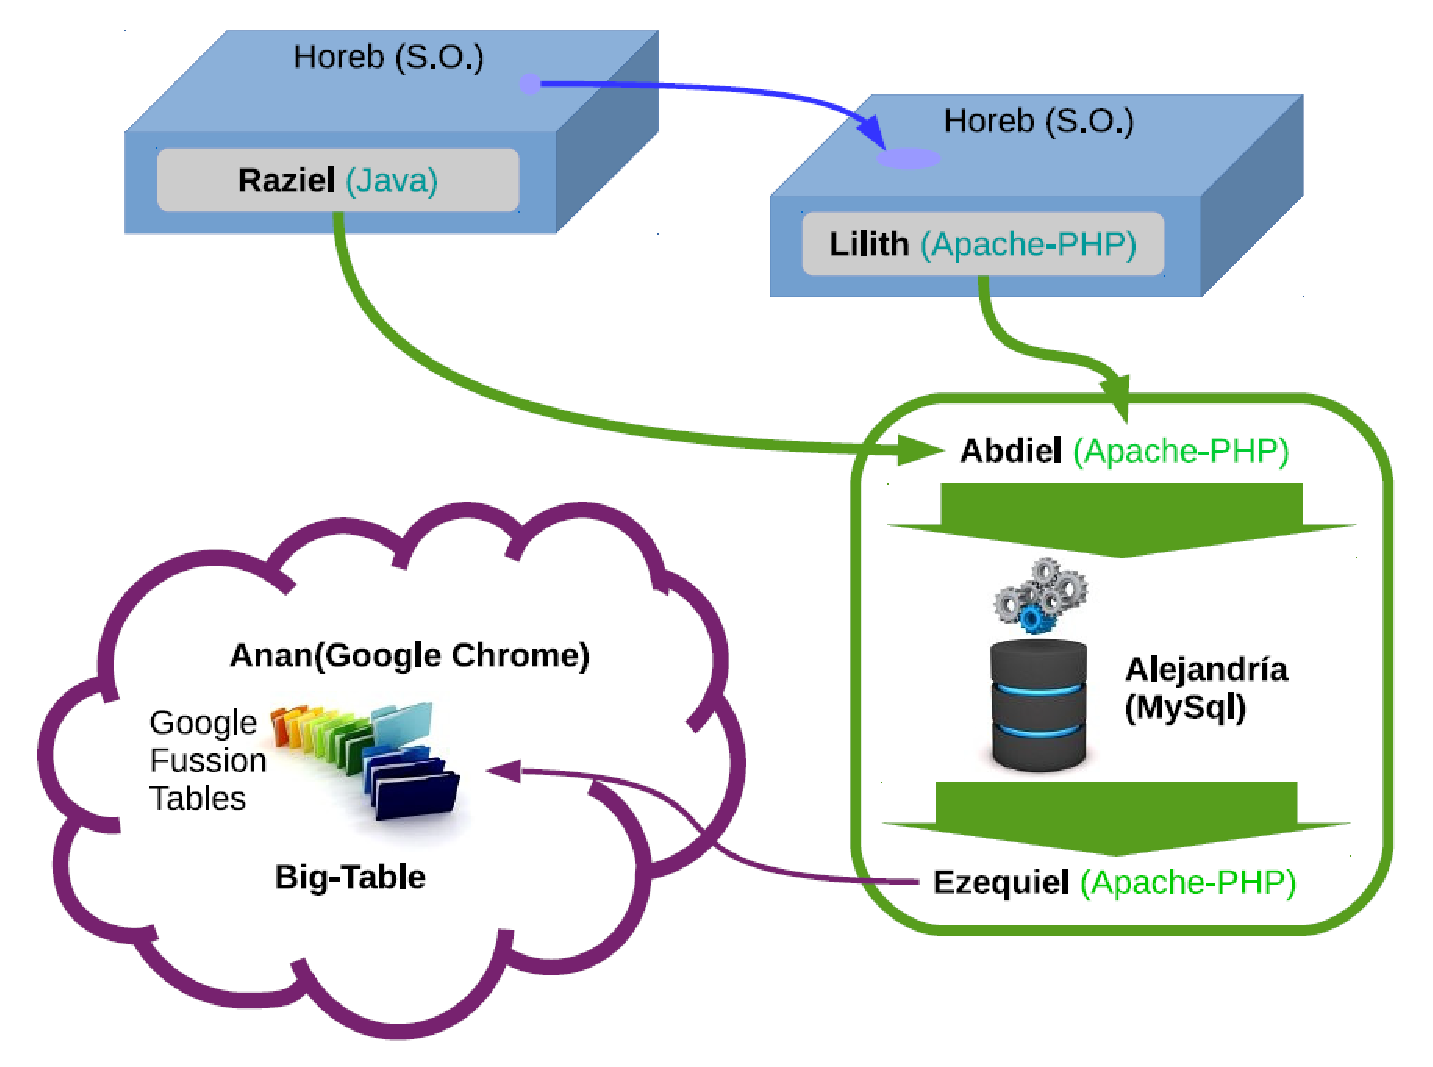
\includegraphics[scale=0.4]{imgs/mobywit.eps}
		\caption{MOBYWIT Monitoring system architecture}
	\label{fig:mobywit}
	\end{center}
\end{figure}
% Antonio - TODO - Pasar la imagen a ingl�s (S.O. -> O.S.)

As it can be seen in that figure, there are six main parts in the software layer of the system, which are unidirectionally connected by a strict data flow. Those parts have been named as:
\begin{itemize}

\item \textit{Raziel}: This module is in charge of the detection of BT and WiFi devices as well as of their identification (extracting and encrypting the MAC) and the periodic submission of this information to the server. It runs on the device and has been implemented in Java.

\item \textit{Lilith}: This module acts as a gateway between the network of devices and the server. It allows the communications between nodes and between them and external networks. This component is also run on every device and implemented in PHP.

\item \textit{Abdiel}: This component implements a set of services for accessing the devices from `outside' (mainly for activate/deactivate or update them). In addition, it performs the storage of gathered data (in blocks) in the server database. It is also implemented in PHP.

\item \textit{Alejandr�a}: This is the system database. It is a MySQL instance placed in a local server. It is optimised using b-tree indexes, stored procedures, table partitioning and temporally memory tables to provide a close to real-time processing and data service.

\item \textit{Ezequiel}: This module is responsible for the publication of data in a cloud-based storage. It includes data mining, machine learning and forecast techniques to process these data in order to publish interesting or useful information about them.

\item \textit{Anan}: This is the cloud-based storage and services. It is based on Google technology so Anan stores and manages the data in a NoSQL format, by means of Google Fusion Tables. It also offers advanced visualisation methods to be more usable and attractive to the end-user of the system.

\end{itemize}

In addition, and as it is shown in Figure \ref{fig:mobywit}, the device runs a specific Operative System, called \textit{Horeb}, which is a modification of the original Raspbian 3.10.24, adapted by MOBYWIT system designer to be more robust (to power fails, for instance) and reliable.

There are several configuration parameters in the system, which set important parts of the functionality, such as the intensity threshold to collect a received WiFi signal, or time limits to consider a device as obsolete or out of the range of the device.

Every detected `pass-by' or mobility `event' is associated with a detection time, obtained by NTP (Network Time Protocol). These `events' are stored initially in the device's memory. After some time (also set in a parameter) the information is sent, in blocks, to the server, to avoid an overuse/saturation of the network.

MOBYWIT system is tested in four different scenarios, described in the
following sections, in order to prove its value in different urban
problems. 

\subsection{Data validation using other sources of data}

Different metrics will be used to obtain a correct correlation between the number of detected devices and the real number detected by the loop detectors. 

\begin{itemize}
\item {\em Total ratio}: ratio between the total number of vehicles detected by the DGT and the total number of vehicles detected by our device.
\item {\em Mean ratio}: as the maximum granularity of the data provided by the DGT is 15 minutes, the sum of all ratios between the DGT data and our data in each 15 minute section has been divided by the total number of sections to calculate the average.
\item {\em Median ratio}: instead the average ratio as in previous metric, this one uses the median of all ratios.
\item {\em Mean by quarter ratio}: this metric calculates a vector of ratios separated by quarter of hour during the day, instead obtaining a global ratio for all data. An average ratio per quarter per hour in the vector is calculated taking into account all the ratios of that quarter during all the days we have data.
\item {\em Median by quarter ratio}: as in the previous metric, this one uses a vector of ratios per quarter of hour, but every element is calculated using the median, instead the average.
\end{itemize}


Table \ref{tab:ratiosDGT} shows the obtained ratios. To simplify the data analysis and discussion only the data of one node (1010) are shown. Results show that our device detects one vehicle per approximately 19 detected by the DGT, according Total, Mean and Median ratios. However, best results in MAE and MAPE are attained obtaining ratios dividing by quarter. Therefore, for the rest of the paper this ratio has been chosen, as we need to deal with absolute values to perform forecasting analysis later.

\begin{table}[htb]
\centering
\resizebox{12cm}{!}{
\begin{tabular}{|l|l|l|l|l|l|}
\hline
			 &RATIO	  & MAE    &   MAPE   & MSE    & RMSE \\
 \hline
Total Ratio  & 17.230 &   60.373 & 36.265 & \textbf{7371.579}  & \textbf{85.857} \\
Mean Ratio   & 20.792 &   72.323 & 43.443 & 11216.070 & 105.905 \\
Median Ratio & 18.2 &    62.454  & 37.515 & 8060.136  & 89.778 \\
Mean By Quarter of Hour Ratio &   Depends on the hour  & 66.791 & 40.120 & 9890.978 & 99.453 \\
Median By Quarter of Hour Ratio & Depends on the hour  & \textbf{58.326} & \textbf{35.035} & 7617.613 & 87.278 \\
\hline

\end{tabular}
}
\caption{Different ratios between the DGT data and the data gathered by MOBYWIT in node 1010.}
\label{tab:ratiosDGT}
\end{table}


Figure \ref{fig:dgtRatios} shows the number of devices of the node 1010, applying the chosen correction ratio. As it can be seen, certain correlation exists. However, different peaks appear in the figure, being those elements the product of detecting few devices in comparison with the DGT.



\begin{figure}[htb]
	\begin{center}
		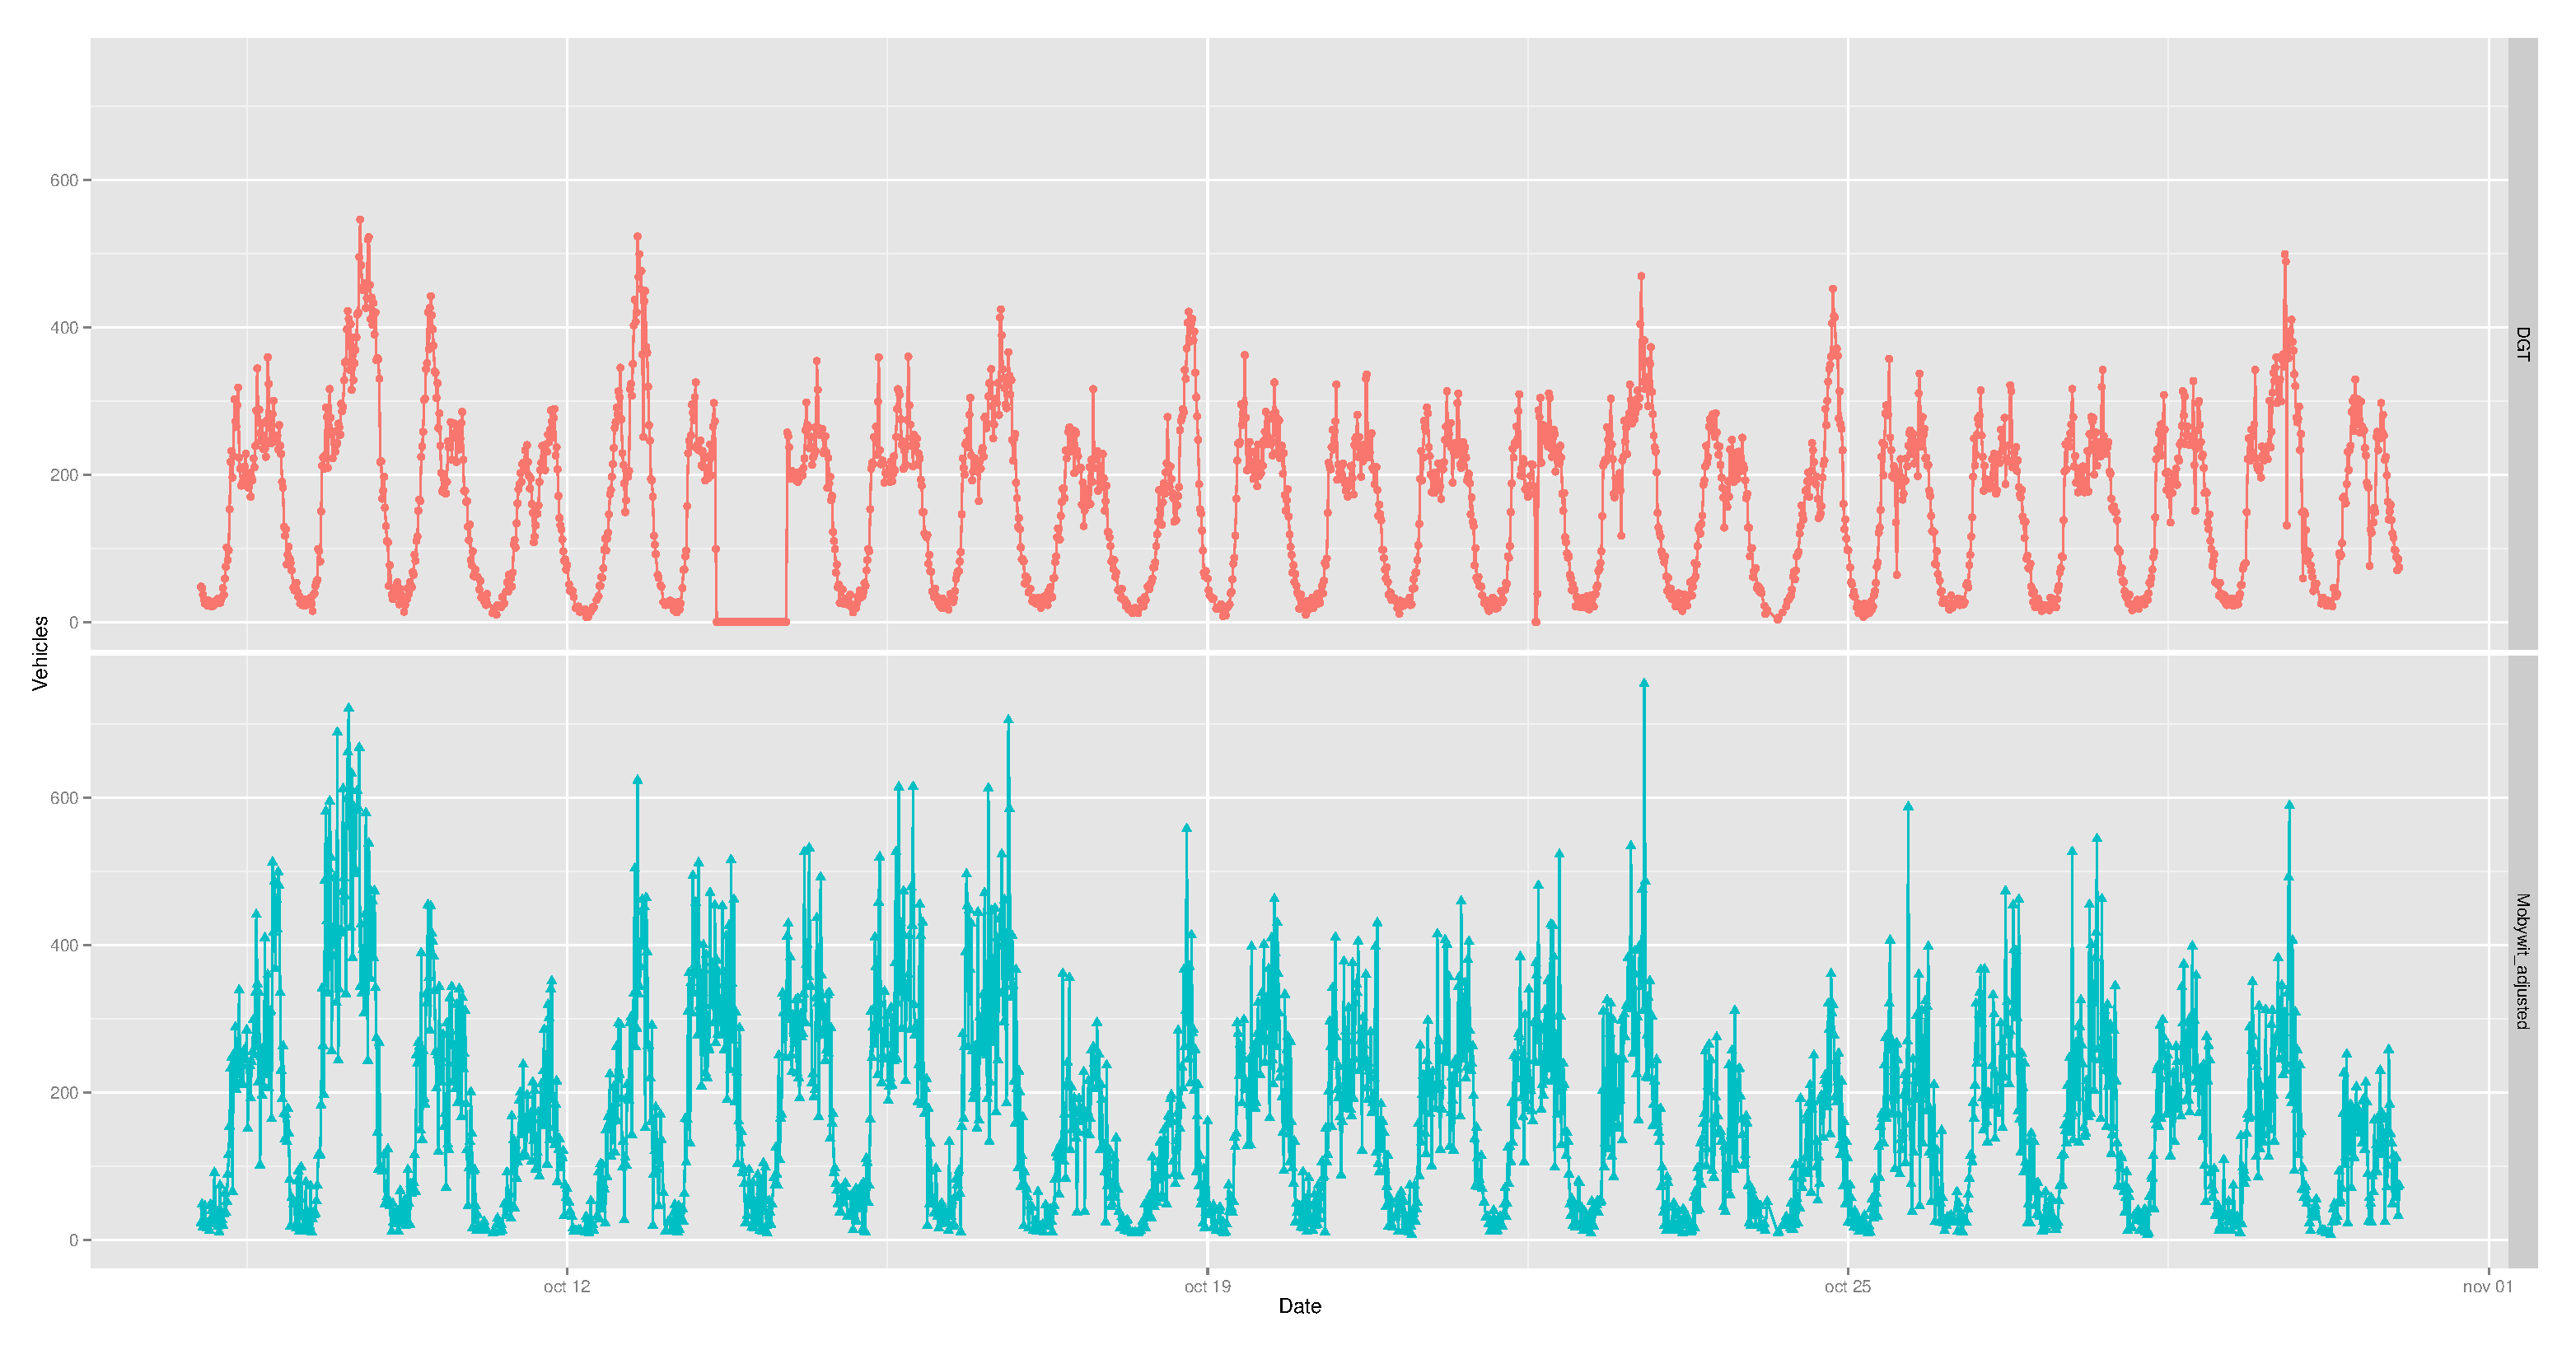
\includegraphics[scale=0.22]{imgs/petra_graph_DGT-Mobywit-mended.eps}
		\caption{Devices detected by DGT and detected by our device (node 1010) applying the correction ratio (median by quarter). Note: no DGT data available during October 14th.}
	\label{fig:dgtRatios}
	\end{center}
\end{figure}



%----------------------------------------------------------------------------
%%%%%%%%%%%%%%%%%%%%%%%%%%%%%%%   CONCLUSIONS  %%%%%%%%%%%%%%%%%%%%%%%%%%%%%%%
%----------------------------------------------------------------------------

\section{Conclusions}
\label{sec:conclusions}

In this work, MOBYWIT, a novel monitoring and tracking system which gathers mobility data from people and vehicles has been presented. Some of its applications have been shown, using the data collected by the system to address different issues in a city in order to make it `smarter'.
Thus, four different scenarios have been studied:

\begin{itemize}
    \item A discotheque, which has been used as a `stress test' for the system and also to address issues on marketing, energetic efficiency and security in the building, considering the mobility of people inside it on different nights. Clustering methods have been applied in order to visualise and extract interesting knowledge about people's movements and recurrences to the disco.
    \item A public building of the University of Granada, in which students', teachers' and other staff's movements have been analysed using origin/destination matrices with a similar objective than before: security, access improvements and (possibly) marketing reasons.
    \item An interurban road, where the traffic flows have been studied and contrasted with real traffic data, using statistical methods to estimate the real number of vehicles. Forecast techniques have been applied with very good results in the short-term. The forecast has been applied with both real traffic values and captured values with MOBYWIT, adjusted with the calculated ratio of real vehicles / detected vehicles. Moreover, a matrix to show the average travel duration between nodes has been calculated.
    \item An urban street, which is one of the main arteries of the city of Granada, so it is usually collapsed. A statistical analysis has been conducted to study the traffic flows, detecting possible jams. This information could be potentially used in order to improve the light signal synchronisations in that street.
\end{itemize}

The aim of the work was to show that the results of these studies could be the basis for solving the commented issues, as well as to prove the value and reliability of the presented system. 

Since this paper is a kind of `proof of concept' for MOBYWIT, several future lines of research are open.
Firstly, a deeper study on every issue addressed in the work can be done, focusing on every scenario, considering bigger amounts of data and applying some other techniques, which would improve the quality of the results. Moreover, we could aim to improve the methods of the state of the art for different problems, such as traffic forecast, for instance, but considering our gathered real data, offering these data as benchmarks for the scientific community.

Also, some other problems in the city could be addressed using MOBYWIT devices, for instance, analysing people's and traffic mobility in the city, in order to improve services (to the tourists, for instance), conduct geo-marketing analyses \cite{Flyers-GeoMarketing,LaMarca-GeoMarketing}, increase the security mechanisms, or improve the public transport system.
This would require the deployment of several devices around the city, in order to better build mobility graphs, origin/destination matrices and other mobility models.

The system itself has some flaws or weak points that could be improved, such as avoiding the overlapping between detections in two different nodes (using unidirectional antennas or some kind of filters or blocking panels).

Another point of improvement could be the use of Time Series Forecast techniques in order to complete `holes' in the detected `events' when there is a power cutoff on a device.

%%%%%%%%%%%%%%%%%%%%%%%%%%%%%  ACKNOWLEDGEMENTS %%%%%%%%%%%%%%%%%%%%%%%%%%%%%%%%

\section*{Acknowledgements}

This work has been supported in part by projects EPHEMECH (TIN2014-56494-C4-3-P, Spanish Ministry of Economy and Competitivity), PETRA (SPIP2014-01437, funded by Direcci�n General de Tr�fico), PYR-2014-17 (GENIL project, awarded by CEI-BIOTIC Granada), and MOSOS (This work has been supported by the project with reference PRY142/14, which has been granted by Fundaci�n P�blica Andaluza Centro de Estudios Andaluces in the call 'IX Convocatoria de Proyectos de Investigaci�n). We also thank the DGT and local council of Granada city, and their staff and researchers for their dedication and professionalism. 


% ---------------------- BIBLIOGRAF�A -----------------------

\bibliographystyle{elsarticle-num}
\bibliography{mobility}


% ------------------------- AP�NDICE -----------------------


\section{Appendix} 
\label{appendix}

This appendix presents additional information about the scenarios, such as the geographical position of the nodes and a comment about them, or some graphs showing the distribution of the gathered data.

\begin{table}[H]
\centering
\resizebox{12cm}{!}{
\begin{tabular}{|c|c|p{5cm}|c|c|}
\hline
ID   &  Location & Latitude & Longitude \\ \hline
102	 &  DISCO Terrace & -Non-Allowed- & -Non-Allowed- \\ \hline
112	 &  DISCO Main room  & -Non-Allowed- & -Non-Allowed-  \\ \hline
122	 &  DISCO Minor room 1& -Non-Allowed- & -Non-Allowed- \\ \hline
132	 &  DISCO Ticket office & -Non-Allowed- & -Non-Allowed- \\ \hline
142	 &  DISCO Minor room 2& -Non-Allowed- &  -Non-Allowed- \\ \hline
\end{tabular}
}
\caption{Location of the devices for Discotheque scenario. The exact coordinates cannot be shown due to privacy reasons in a contract.}
\label{tab:nodosDisco}
\end{table}

\begin{table}[H]
\centering
\resizebox{12cm}{!}{
\begin{tabular}{|c|c|p{5cm}|c|c|}
\hline
ID   &  Location & Latitude & Longitude \\ \hline
42	 &  ETSIIT Parking & 37.197377 & -3.6247944\\ \hline
52	 &  ETSIIT Main access of Students& 37.196729 &  -3.62435722\\ \hline
62	 &  ETSIIT Main access of Staff & 37.196928 & -3.6244201\\ \hline
\end{tabular}
}
\caption{Location of the devices for the Building of the University scenario.}
\label{tab:nodosETSIIT}
\end{table}

\begin{table}[H]
\centering
\resizebox{12cm}{!}{
\begin{tabular}{|c|c|p{5cm}|c|c|}
\hline
ID   & Province & Location & Latitude & Longitude \\ \hline
1010 & Granada  & A-44 K.P. 118+300 increasing direction (link A-44 K.P. 118+300 with A-92 K.P. 241+000) & 37.241668  & -3.6526 \\ \hline
1020 & Granada  & A-92 K.P. 294+300 increasing direction  & 37.318763 & -3.137978 \\ \hline
1030 & Granada  & A-92 K.P. 344+950, increasing direction & 37.141298 & -2.710871 \\ \hline
1040 & M{\'a}laga  & A-7  K.P. 241+800, decreasing direction (Link A-7 K.P. 241+800 with A-45 K.P. 142+400) &  36.757427 & -4.426879 \\ \hline
1050 & M{\'a}laga  & A-45 K.P. 121+700, decreasing direction & 36.910454 & -4.444769 \\ \hline
1060 & Granada & A-92 K.P. 177+900, decreasing direction (Link A-92 with A-92M) & 37.136209 & -4.282619 \\ \hline
\end{tabular}
}
\caption{Location of the devices for the highway traffic scenario (K.P. = Kilometric Point).}
\label{tab:nodosDGT}
\end{table}


\begin{table}[H]
\centering
\resizebox{12cm}{!}{
\begin{tabular}{|c|c|p{5cm}|c|c|}
\hline
ID   & Province & Location & Latitude & Longitude \\
\hline
A	 & Granada & Dr. Ol�riz Street & 37.188187 & -3.607241\\ \hline
B	 & Granada & Dr. Ol�riz Street & 37.186997 & -3.607882\\ \hline
\end{tabular}
}
\caption{Location of the devices for the city traffic scenario.}
\label{tab:nodosCity}
\end{table}


\end{document}
